% !TEX root =  ../main_manuscript.tex 
\section{Demonstration of Personalized Schedules}
\label{sec:results}
We return to the prostate cancer active surveillance dataset, PRIAS, described in Section~\ref{sec:introduction}. The clinical data consists of longitudinal PSA (continuous; ng/mL) and DRE (binary; tumor palpable or not) measurements, patient age at baseline, history of biopsies, and interval-censored times of cancer progression. The event of interest is cancer progression. We aim to use the accumulated clinical data to build joint models that can be utilized for creating personalized biopsy schedules in future PRIAS patients. 

The current PRIAS protocol for biopsies is fixed biopsies at year one, four, seven, and ten of follow-up, and every five years after that. Additional annual biopsies are scheduled if a patient's PSA doubling-time~\citep{bokhorst2015compliance} is high. The PSA is measured as per a fixed schedule, quarterly for the first two years, and semi-annually after that. The DRE is also measured semi-annually. The dataset is described in more detail in Web-Appendix~B.

\subsection{Fitting the Joint Model to the PRIAS Dataset}
We first fit a joint model to the accumulated clinical data, with $\log_2(\mbox{PSA} + 1)$ transformed PSA~\citep{lin2000latent,pearson1994mixed}, and DRE as longitudinal measurements, and cancer progression as the event (Web-Appendix~B for exact specification). For PSA we utilize a linear mixed-effects sub-model wherein PSA profiles are modeled non-linearly over follow-up using B-splines~\citep{de1978practical}. For DRE, we utilize a logistic mixed-effects sub-model. To link the longitudinal sub-models for the PSA and DRE with the relative-risk sub-model for cancer progression, we include three features of the longitudinal outcomes in the relative-risk sub-model. Specifically, the hazard of cancer progression at time $t$ depends on the fitted instantaneous $\log_2(\mbox{PSA} + 1)$ value at time $t$, the estimated instantaneous $\log_2(\mbox{PSA} + 1)$ velocity at $t$, and fitted log-odds of having a DRE indicating a palpable tumor at $t$. We estimated the parameters of our model under the Bayesian framework using the R package \textbf{JMbayes}~\citep{rizopoulosJMbayes}.  

The follow-up period of PRIAS is limited currently. Hence, our joint model is able to predict the cumulative-risk of progression only until the year ten of follow-up. The cumulative-risk of progression at year ten in PRIAS is 50\% (see Web-Figure.). We found that the strongest predictor for progression in our model is $\log_2(\mbox{PSA} + 1)$ velocity. Specifically, for an increase in fitted $\log_2(\mbox{PSA} + 1)$ velocity from -0.03 to 0.15 the adjusted hazard ratio of progression was 1.6 (95\%CI: 1.45--1.78). Detailed parameter estimates are in Web-Appendix~B.

\subsection{Personalized Schedules for a Demonstration Patient}
We utilized the joint model fitted to the PRIAS dataset to schedule biopsies in a real PRIAS patient (Figure~\ref{fig:demo_schedule}), starting from his current visit at year five, until a horizon of year ten of follow-up. The cumulative-risk of progression of this patient at his current visit is 6\% whereas at ten years it is 16.5\%. Thus, the patient is predicted to progresses slowly. Consequently, risk based personalized schedules in Panel~B of Figure~\ref{fig:demo_schedule} planned much less biopsies than the standard annual schedule. At the same time, the expected time delay in detection of progression in personalized schedules is also less than one year (maximum delay possible with annual schedule). It is important to note that for a fair comparison of expected time delay, we scheduled a compulsory biopsy at the horizon of ten years in all schedules. In addition, between consecutive biopsies we maintained a recommended minimum gap of one year~\citep{bokhorst2016decade}.

\begin{figure}
\centerline{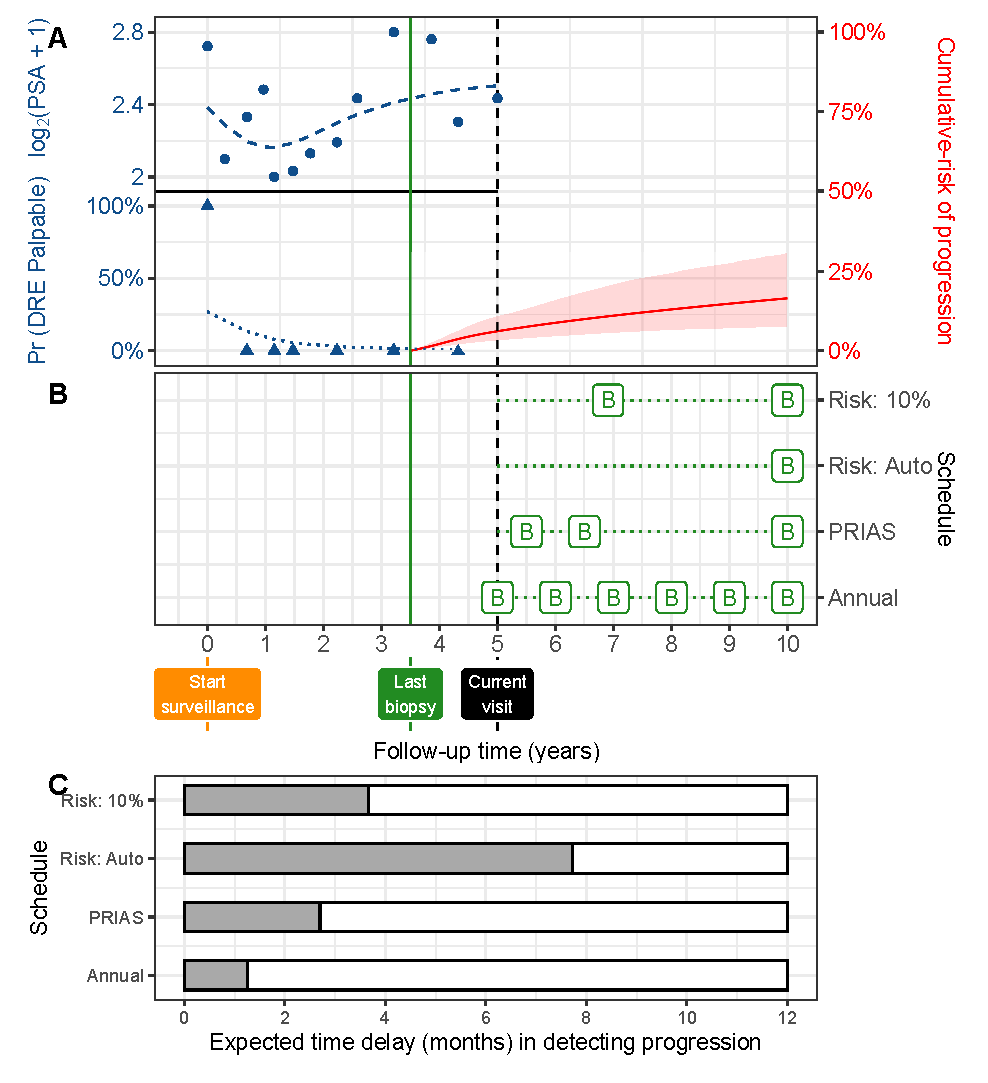
\includegraphics{images/demo_schedule.eps}}
\caption{\textbf{Demonstration of personalized schedules for a real PRIAS patient:} In \textbf{Panel~A}: Time of last negative biopsy is year 3.5 (vertical green solid line). Longitudinal data is repeated DRE (blue triangles) and PSA measurements (blue circles). Current visit is year five (vertical black dashed line). Estimated cumulative-risk profile is shown with a solid red line (95\%CI is shaded). It is 6\% at the current visit and 16.5\% at year ten (horizon). In \textbf{Panel~B}, we visualize different biopsy schedules, with a `B' indicating a biopsy. \textbf{Risk: 10\%} and \textbf{Risk: Auto} are personalized biopsy schedules using a fixed risk threshold $\kappa=10\%$, and automatically chosen $\kappa_a$ (Equation~\ref{eq:kappa_choice}), respectively. \textbf{PRIAS} and \textbf{Annual} denote the PRIAS biopsy schedule (paragraph~2 of Section~\ref{sec:results}) and annual biopsy schedule. \textbf{Panel~C}: For personalized, PRIAS, and annual biopsy schedules we calculate the corresponding expected time delays in detection of progression (Equation~\ref{eq:expected_delay}). A compulsory biopsy at year ten was planned in all schedules for a fair comparison of expected time delay.} 
\label{fig:demo_schedule}
\end{figure}

\subsection{Web-Application}
We implemented our methodology ..